%% LyX 2.3.2 created this file.  For more info, see http://www.lyx.org/.
%% Do not edit unless you really know what you are doing.
\documentclass{article}
\usepackage[utf8]{inputenc}
\usepackage{geometry}
\geometry{verbose,tmargin=2cm,bmargin=2.5cm,lmargin=2.3cm,rmargin=2cm}
\usepackage{array}
\usepackage{verbatim}
\usepackage{units}
\usepackage{multirow}
\usepackage{amsmath}
\usepackage{graphicx}
\usepackage{wasysym}

\makeatletter

%%%%%%%%%%%%%%%%%%%%%%%%%%%%%% LyX specific LaTeX commands.
\newcommand{\noun}[1]{\textsc{#1}}
%% Because html converters don't know tabularnewline
\providecommand{\tabularnewline}{\\}

%%%%%%%%%%%%%%%%%%%%%%%%%%%%%% Textclass specific LaTeX commands.
\newcommand{\lyxaddress}[1]{
	\par {\raggedright #1
	\vspace{1.4em}
	\noindent\par}
}

%%%%%%%%%%%%%%%%%%%%%%%%%%%%%% User specified LaTeX commands.
\usepackage{lipsum}
\usepackage{xr}
\externaldocument{Paper_req-550_SM_V2.0.0}
\usepackage{lineno}
%\usepackage[strings]{underscore} % to include underscores (appearing in bib fields)
%\usepackage[english]{babel} % should go in hand with this to prevent errors (better to escape the underscores)
\usepackage{lineno}
\usepackage{xcolor}
\usepackage{float}
\usepackage{tikz}
\usetikzlibrary{arrows}
%% Strike out display math with tikz
\usetikzlibrary{calc}
%\newcommand{\lyxmathsout}[1]{%
%  \tikz[baseline=(math.base)]{
%    \node[inner sep=0pt,outer sep=0pt](math){#1};
%    \draw($(math.south west)+(2em,.5em)$)--($(math.north east)-(2em,.5em)$);
%  }
%}
\newcommand{\bs}[1]{\boldsymbol{#1}}
\newcommand{\add}[1]{\textcolor{red}{#1}}
\newcommand{\oran}{\mathrm{o}}
\newcommand{\g}{\mathrm{g}}
\newcommand{\X}{\mathrm{X}}
\newcommand{\Y}{\mathrm{Y}}
\newcommand{\PP}{\mathrm{P}}
\newcommand{\EE}{\mathrm{E}}
\newcommand{\HH}{\mathrm{H}}
\newcommand{\DD}{\mathrm{D}}
\newcommand{\RR}{\mathrm{R}}
\newcommand{\A}{\mathrm{A}}
\newcommand{\I}{\mathrm{I}}
\newcommand{\M}{\mathrm{M}}

\newcommand{\sh}{\mathrm{sh}}
\newcommand{\nullm}{\mathrm{null}}
\newcommand{\intv}{\mathrm{intv}}
\newcommand{\family}{\mathrm{visit}}
\newcommand{\care}{\mathrm{care}}
\newcommand{\Exp}{\mathrm{exp}}
\newcommand{\onset}{\mathrm{onset}}

\makeatother

\begin{document}
\title{Empowering the crowd: Feasible strategies \\
 for epidemic management in high-density informal settlements.\linebreak{}
 The case of COVID-19 in Northwest Syria}
\author{Alberto Pascual-García$^{(1,*)}$, Jordan Klein$^{(2)}$, Jennifer
Villers$^{(3,\land)}$, \\
 Eduard Campillo-Funollet$^{(4,\wedge)}$, Chamsy Sarkis$^{(5)}$}
\maketitle

\lyxaddress{\begin{center}
(1) Institute of Integrative Biology. ETH-Zürich. Zürich, Switzerland.
\\
 (2) Office of Population Research. Princeton University. Princeton,
NJ, USA. \\
 (3) Princeton Environmental Institute. Princeton University. Princeton,
NJ, USA. \\
 (4) Genome Damage and Stability Centre. University of Sussex. Brighton,
United Kingdom. \\
 (5) Pax Syriana Foundation. Valetta, Malta. \\
 ($\land$) Equal contribution. \\
 ({*}) correspondence: alberto.pascual@env.ethz.ch.\\
Universitätstrasse 16. 8005, Zürich (Switzerland). Tel. +41 44 632
89 22
\par\end{center}}
\begin{abstract}
More than 1 billion people live in informal settlements worldwide,
where precarious living conditions pose unique challenges to managing
a COVID-19 outbreak. Taking Northwest Syria as a case-study, we simulated
an outbreak in high-density informal Internally Displaced Persons
(IDP) camps using a stochastic Susceptible-Exposed-Infectious-Recovered
model. Expanding on previous studies, taking social conditions and
population health/structure into account, we modeled several interventions
feasible in these settings: moderate self-distancing, self-isolation
of symptomatic cases, and protection of the most vulnerable in “safety
zones”. We considered complementary measures to these interventions
that can be implemented autonomously by these communities, such as
buffer zones, health-checks, and carers for isolated individuals,
quantifying their impact on the micro-dynamics of disease transmission.
All interventions significantly reduce outbreak probability and some
of them reduce mortality when an outbreak does occur. Self-distancing
reduces mortality by up to 35\% if contacts are reduced by 50\%. A
reduction in mortality by up to 18\%can be achieved by providing 1
self-isolation tent per 8 people. Protecting the most vulnerable in
a safety zone reduces the outbreak probability in the vulnerable population
and has synergistic effects with the other interventions. Our model
predicts that a combination of all simulated interventions may reduce
mortality by morethan 90\% and delay an outbreak’s peak by almost
two months. Our results highlight the potential for non-medical interventions
to mitigate the effects of the pandemic. Similar measures may be applicable
to controlling COVID-19 in other informal settlements, particularly
IDP camps in conflict regions, around the world.
\end{abstract}
\bigskip{}

\textbf{Keywords:} COVID 19 \textbar{} Epidemiology \textbar{} community-led
interventions \textbar{} SIR models \textbar{} Internally Displaced
Persons \textbar{} Syria \textbar{} Refugees

\medskip{}

\textbf{Abbreviations: }IDP: Internally Displaced Persons \textbar{}
NWS: Northwest region of Syria \textbar{} IFR: Infection fatality
rate \textbar{} ICU: Intensive care unit \textbar{} IBM: Individual
based models

\medskip{}

\textbf{Word count:} 5898

\newpage{}

\subsection*{Key questions}

\subsubsection*{What is already known?}
\begin{itemize}
\item Since the onset of the COVID-19 pandemic, many studies have provided
evidence for the effectiveness of strategies such as social distancing,
testing, contact tracing, case isolation, use of personal protective
equipment/facemasks and improved hygiene to reduce the spread of the
disease. These studies underlie the recommendations of the World Health
Organisation, but their implementation is contingent on local conditions
and resources.
\item Mathematical modelling is the basis of many epidemiological studies
and has helped inform policymakers considering COVID-19 responses
around the world. Nevertheless, only a limited number of studies have
applied these models to informal settlements.
\end{itemize}

\subsubsection*{What are the new findings?}
\begin{itemize}
\item We developed a mathematical model to study the dynamics of COVID-19
in Syrian IDP camps, elaborating on previous efforts done in similar
settings by explicitly parameterizing the camps’ demographics, living
conditions and micro-dynamics of interpersonal contacts in our modelization.
\item We designed interventions such as self-distancing, self-isolation
and the creation of safety zones to protect the most vulnerable members
of the population, among others, through conversations with camp managers
with on-the-ground knowledge of what interventions would be feasible
and have community buy-in.
\item Our results show how low-cost, feasible, community-led non-medical
interventions can significantly mitigate the impact of COVID-19 in
Northwest Syrian IDP camps.
\end{itemize}

\subsubsection*{What do the new findings imply?}
\begin{itemize}
\item Our model represents a step forward in the much-needed search for
epidemiological models that are sufficiently flexible to consider
specific social questions. The model can also help inform similar
interventions in refugee camps in conflict-torn regions, and potentially
be adapted to other informal settlements and vulnerable communities
around the world.
\end{itemize}
\newpage{}

\section*{Introduction}

\begin{comment}
The COVID-19 pandemic is intensifying in the developing world \cite{Guardian1M}.
In Africa, SARS-CoV-2 has been spreading from urban areas to informal
settlements \cite{WHO_AfricaMarks6months}. With more than 1 billion
people living in informal settlements worldwide, urgent action is
needed to contain the virus in these settings, a task which necessarily
involves the engagement of the communities living in them \cite{wilkinson_local_2020}.
\end{comment}

The spread of airborne infectious diseases with pandemic potential
in regions immersed in protracted armed conflicts, where large portions
of their populations have become displaced, is an important challenge
\cite{san_humanitarian_2020}. When the displaced population exceeds
official resettlement and refugee camp capacity, Internally Displaced
Persons (IDPs) must live in informal settlements (hereafter named
``camps''). These regions must contend with the public health challenges
resulting from violence \cite{abbas_migrant_2018}, the deterioration
of health-systems \cite{hill_conflict_2010}, especially of critical
care \cite{sahloul_war_2016}, and the breakdown of essential public
infrastructure such as water and sanitation systems \cite{sikder_water_2018}.
Urgent action is needed to contain the spread of disease in these
settings, a task which necessarily involves the engagement of the
communities living in them \cite{wilkinson_local_2020}.

This study focuses on the spread of COVID-19 inNorthwest region of
Syria (NWS): a relatively small geographical area with 4.2 million
people, of which 1.15 million (27.4\%) are IDPs living in camps \cite{Health_directorate},
and where the number of cases increased twenty-fold between September
8th and October 20th, 2020 \cite{UNOCHA_collapse}. The health status
of households in camps in NWS is poor; 24\% have a member with a chronic
disease, of whom 41\% have no access to medicines \cite{noauthor_syria_nodate}.
As in other conflict regions, the political instability in NWS hinders
coordinated public health actions, and the ongoing movements of IDPs
create ample opportunity for infectious disease transmission, while
making contact tracing interventions infeasible.

To investigate feasible COVID-19 prevention interventions in the camps,
we considered a Susceptible-Exposed-Infectious-Recovered model similar
to the one presented by Gatto \emph{et al.} \cite{gatto_spread_2020},
in which the camps' populations are divided into classes reflecting
their estimated age-structures and comorbidity prevalence. We use
this model to propose various interventions aimed at reducing the
number of contacts within and between population classes in general,
and with symptomatic individuals in particular. We paid special attention
to how the living conditions in informal camps inform the assumptions
underlying our proposed interventions, a question often neglected
\cite{rhodes_Model2context_2020}. We modeled interventions previously
proposed for African cities \cite{vanzandvoort2020}, such as self-distancing,
isolation of symptomatic individuals and the creation of a 'safety
zone' in which more vulnerable members of the population are protected
from exposure to the virus.

Building upon the approach used to model the impact of these interventions
in African cities, our model includes a parameterization of the contacts
each individual has per day \cite{vanzandvoort2020}. We further elaborate
upon this approach by making a more explicit representation of contacts
and other parameters in the model. We consider the micro-dynamics
of contacts, the time that individuals take to recognize their symptoms
before self-isolating, the effect of having carers to attend to isolated
individuals, and the existence of a buffer zone in which exposed and
protected population classes can interact under certain rules. We
examine a potential worst-case scenario in which there is no access
to any healthcare facility. Since empowering local communities in
conflict regions to understand how to control diseases like COVID-19
is possibly the most (and perhaps only) effective way to minimize
its spread, our models are of utmost importance for informing the
implementation of realistic interventions in these regions.

\section*{Methods}

\subsection*{The model}

We consider a model simulating a viral outbreak in a single camp over
a 12-month period inspired by those proposed by Gatto \emph{et al.}
and Bertuzzo \emph{et al.} \cite{gatto_spread_2020,bertuzzo_geography_2020}
(see Fig. \ref{fig:Diagram}). The model is adapted to the context
of NWS IDP camps and is divided into compartments containing individuals
at different possible stages along the disease's progression, governed
by the following set of differential equations:

\begin{gather}
\dot{S}_{i}=-\lambda_{i}S_{i}\label{eq:System1}\\
\dot{E}_{i}=\lambda_{i}S_{i}-\delta_{\EE}E_{i}\\
\dot{P}_{i}=\delta_{\EE}E_{i}-\delta_{\PP}P_{i}\\
\dot{A}_{i}=(1-f)\delta_{\PP}P_{i}-\gamma_{\A}A_{i}\\
\dot{I}_{i}=f\delta_{\PP}P_{i}-(l_{i}\gamma_{I}+h_{i}\eta+g_{i}\alpha)I_{i}\\
\dot{H}_{i}=h_{i}\eta I_{i}-\gamma_{\HH}H_{i}\\
\dot{R}_{i}=\gamma_{\A}A_{i}+l_{i}\gamma_{\I}I_{i}+(1-\sigma)\gamma_{\HH}H_{i}\\
\dot{D_{i}}=g_{i}\alpha I_{i}+\sigma\gamma_{\HH}H_{i}\label{eq:System8}
\end{gather}

The susceptible population ($S_{i}$) becomes exposed at rate $\lambda_{i}$,
while exposed individuals ($E_{i}$) progress through the latent period
at rate $\delta_{\EE}$ to a preclinical infectious stage ($P_{i}$),
which then progresses to (at rate $\delta_{\PP}$) either a a clinical
(symptomatic, $I_{i}$, with probablity $f$) or subclinical (asymptomatic,
$A_{i}$, with probability $1-f$) infectious stage. Asymptomatic
cases recover ($R_{i}$) at rate $\gamma_{\A}$. Symptomatic cases
have 3 potential outcomes: mild cases will recover at rate $\gamma_{\I}$,
severe cases will progress to an extended infectious period during
which they require hospitalization ($H_{i}$) at rate $\eta$, while
critical cases requiring intensive care unit (ICU) care will die ($D_{i}$)
at rate $\alpha$. Finally, since the fate of individuals in the hospitalized
compartment is uncertain if healthcare is not available, we run simulations
considering two possibilities: either all recover ($\sigma=0$), or
all die ($\sigma=1$) (see section Epidemiological severity assumptions).
The specific values for the parameters are presented in Table \ref{tab:FixedParams}.

While we introduced the model as a classical system of ordinary differential
equations (Eqs. \ref{eq:System1}--\ref{eq:System8}) we considered
a stochastic implementation \cite{engbert_chanceChaos_1994}, with
an integer description of the population in which a state is encoded
in a vector $X=(S,E,P,I,A,H,R,D)^{t}$, with the total population
size conserved throughout the simulation $N=S+E+P+I+A+H+R+D$. The
possible transitions between states of the system are shown in Fig.
\ref{fig:Diagram}, where an arrow indicates transitions in which
the source compartment transfers one individual to the target compartment.
The mean transition rates corresponding to each transition are displayed.
The system then evolves following a continuous-time Markov process
which is simulated following the Gillespie algorithm implemented in
the adaptivetau package \cite{R_adaptivetau}.

\begin{figure}[h]
\begin{centering}
\tikzstyle{int}=[draw, fill=blue!50, minimum size=2em] 
\tikzstyle{init} = [pin edge={to-,thin,black}] 

\begin{tikzpicture}[node distance=2.5cm,auto,>=latex']     
	\node [int] (S) {$\dot{S_i}$};     
	\node (E) [int, right of=S] {$\dot{E_i}$};     
	\node (P) [int, right of=E] {$\dot{P_i}$};   
	\node (blank) [right of=P, coordinate]{};  
	\node (I) [int, below of=blank] {$\dot{I_i}$}; 
	\node (A) [int, above of=blank] {$\dot{A_i}$}; 
	\node (H) [int, right of=I] {$\dot{H_i}$}; 
	\node (R) [int, right of=blank] {$\dot{R_i}$}; 
	\node (D) [int, below of=H] {$\dot{D_i}$}; 
	\path[->] (S) edge node {$\lambda_iS_i$} (E);     
	\path[->] (E) edge node {$\delta_\EE E_i$} (P);    
	\path[->] (P) edge node [anchor=center, left, midway] {$f\delta_\PP P_i$} (I);   
	\path[->] (I) edge node [anchor=center, below, midway] {$h_i{\eta}I_i$} (H);   
	\path[->] (I) edge node [anchor=center, left, pos=0.7] {$\l_i \gamma_\I I_i$} (R);   
	\path[->] (A) edge node [anchor=center, right, midway] {$\gamma_\A A_i$} (R);   
	\path[->] (P) edge node [anchor=center, left, midway] {$(1-f)\delta_\PP P_i$} (A);  
	\path[->] (I) edge node [anchor=center, left, midway] {$g_i{\alpha}I_i$} (D);  
	\path[->] (H) edge node [anchor=center, right, midway] {$(1-\sigma)\gamma_\HH H_i$} (R); 
	\path[->] (H) edge node [anchor=center, right, midway] {$\sigma\gamma_\HH H_i$} (D);  
\end{tikzpicture}
\par\end{centering}
\centering{}\caption{\textbf{\label{fig:Diagram}Diagram of the model. }The model considers
the following compartments: susceptible (S), exposed (E), infectious-presymptomatic
(P), infectious-asymptomatic (A), infectious-symptomatic (I), infectious-requiring
hospitalization (H), recovered (R) and dead (D).}
\end{figure}


\subsubsection*{Demographic-- and behaviour-classes}

The model splits the population into classes (indexed $i$) to account
for heterogeneity with respect to clinical risk and behaviour. Working
with population classes allows us to encode behavioural assumptions
in the model and strike an appropriate balance between generality,
computational tractability, and the requisite specificity to realistically
evaluate our proposed interventions \cite{funk_BehaviourInModels_2015}.
Moreover, the explicit representation of contacts between and within
population classes allows us to design interventions considering cultural
and context-specific assumptions \cite{rhodes_Model2context_2020}
(see section Interventions and Supplementary Material for details).
Under a null model where no interventions are implemented, the distinctions
between classes are only dependent on age and comorbidity status (hereafter
``demographic-classes''). $h_{i}$, $g_{i}$ and $l_{i}$ are demographic-class
specific parameters, adjusted to ensure that the proportions of symptomatic
cases progressing through each of the 3 potential clinical outcomes
(mild, severe, and critical) are consistent with the literature (see
section Epidemiological severity assumptions).

Under some interventions, the demographic-classes may be subdivided
further into subclasses according to behaviour (``behaviour-classes'').
Consequently, different interventions may require models with different
numbers of classes. We refer to both demographic- and behaviour-classes
generically as ``classes'' (see section Interventions for the modelization
of behaviour-classes).

\begin{table}[h]
\begin{tabular}{|>{\centering}m{0.1\textwidth}|>{\centering}m{0.275\textwidth}|>{\centering}m{0.275\textwidth}|>{\centering}m{0.1\textwidth}|>{\centering}m{0.1\textwidth}|}
\hline 
Parameter & Description & Value & Distribution & Reference\tabularnewline
\hline 
\hline 
$\nicefrac{1}{\delta_{\EE}}+\nicefrac{1}{\delta_{\PP}}$ & Incubation period (days) & 5.2 (95\% CI: 4.1-7.0) & Lognormal & \cite{li2020early}\tabularnewline
\hline 
$\nicefrac{1}{\delta_{\PP}}$ & Presymptomatic infectious period (days) & 2.3 (95\% CI: 0.8-3.8) & Gaussian & \cite{he2020temporal,ashcroft_covid-19_2020}\tabularnewline
\hline 
$\nicefrac{1}{\delta_{\EE}}$ & Latent period (days) & $\left(\nicefrac{1}{\delta_{\EE}}+\nicefrac{1}{\delta_{\PP}}\right)-\nicefrac{1}{\delta_{\PP}}$

(Minimum = .5 days) &  & Derived\tabularnewline
\hline 
$\nicefrac{1}{\gamma_{\I}}$ & Symptomatic infectious period (days) & 7 & \_\_\_ & \cite{he2020temporal,wolfel2020virological}\tabularnewline
\hline 
$\nicefrac{1}{\gamma_{\A}}$ & Asymptomatic infectious period (days) & 7 & \_\_\_ & \cite{he2020temporal,wolfel2020virological}\tabularnewline
\hline 
$\nicefrac{1}{\eta}$ & Time from symptom onset to requiring hospitalization (days) & 7 (IQR: 4-8) & Gamma & \cite{wang2020clinical}\tabularnewline
\hline 
$\nicefrac{1}{\alpha}$ & Time from symptom onset to death (critical cases, days) & 10 (IQR: 6-12) & Gamma & \cite{wang2020clinical}\tabularnewline
\hline 
$\nicefrac{1}{\gamma_{\HH}}$ & Time from requiring hospitalization to recovery/death (days) & 10 (IQR: 7-14) & Gamma & \cite{wang2020clinical}\tabularnewline
\hline 
$f$ & Probability an infectious individual is symptomatic & 0.84 (95\% CI: 0.8-0.88) & Binomial & \cite{byambasuren2020estimating}\tabularnewline
\hline 
$\sigma$ & Indicator of whether hospitalized recover or die & $\sigma\in\{0,1\}$ & \_\_\_ & Assumed\tabularnewline
\hline 
\end{tabular}

\caption{\label{tab:FixedParams}\textbf{Fixed parameters. }See Supplementary
Materials for details.}
\end{table}


\subsection*{Population structure of demographic-classes}

We parameterized the model with data from IDPs in NWS \cite{noauthor_syrian_nodate}.
The population sizes of informal camps are right-skewed, with a mean
of 1212. We simulated camps with populations of 500, 1000 and 2000
individuals. Since interventions tend to be less effective in larger
camps, the results presented refer to simulations with 2000 individuals,
unless otherwise specified. For our demographic-classes, we considered
3 age groups: children (age 1, 0-12 years old), younger adults (age
2, 13-50 yrs) and older adults (age 3, \textgreater 50 yrs). For
ages 2 and 3, we considered two subclasses comprising healthy individuals
and individuals with comorbidities (see Table \ref{tab:PopParams}).

\begin{table*}
\begin{tabular*}{1.1\textwidth}{@{\extracolsep{\fill}}|>{\centering}m{0.08\textwidth}|>{\centering}m{0.09\textwidth}|>{\centering}m{0.07\textwidth}|>{\centering}m{0.15\textwidth}|>{\centering}m{0.12\textwidth}|>{\centering}m{0.15\textwidth}|>{\centering}m{0.12\textwidth}|>{\centering}m{0.09\textwidth}|}
\cline{3-8} \cline{4-8} \cline{5-8} \cline{6-8} \cline{7-8} \cline{8-8} 
\multicolumn{1}{>{\centering}m{0.08\textwidth}}{} &  & \multicolumn{5}{c|}{Demographic-class} & \tabularnewline
\hline 
Parameter & Description & Age 1 (0-12) & Age 2 (13-50)

no comorbidities & Age 2 (13-50)

comorbidities & Age 3 (\textgreater 50)

no comorbidities & Age 3 (\textgreater 50)

comorbidities & References\tabularnewline
\hline 
\hline 
Fraction in class & \_ & 0.407 & 0.471 & 0.0626 & 0.022 & 0.0373 & \noun{\cite{noauthor_syrian_nodate,helpage_international_hidden_2014}}\tabularnewline
\hline 
$c_{i}$ & Mean contacts per day & 25 & 15 & 15 & 10 & 10 & From camp managers\tabularnewline
\hline 
\end{tabular*}

\caption{\label{tab:PopParams}\textbf{Demographic class-specific parameters.}
Estimated proportions of individuals in the population and mean number
of contacts per individual per day for each demographic class. See
Supplementary Materials for derivations.}
\end{table*}


\subsection*{Transmissibility assumptions}

Although individuals in IDP camps share tents with other co-occupants,
whom they may be more likely to infect than occupants of different
tents, we ignore spatial structure in our model and assume a well-mixed
population. This is justified because individuals from different tents
share common spaces (e.g. latrines) and have frequent interactions
with each other, especially among children. Consequently, our following
derivation of the transmissivity parameter itself, $\tau$, is not
spatially explicit.

The rate at which susceptible individuals become exposed is

\medskip{}

\begin{equation}
\lambda_{i}=\sum_{j=1}^{n}\tau C_{ij}\frac{\beta_{\PP}P_{j}+\beta_{\A}A_{j}+\beta_{\I}I_{j}+\beta_{\HH}H_{j}}{N_{j}},\label{eq:lambda}
\end{equation}

\medskip{}

where $C_{ij}$ is the average number of contacts that individuals
of class $i$ have with individuals of class $j$ per day and $N_{j}$
is the total population size of class $j$. We parameterized $C_{ij}$
by multiplying the mean number of total contacts that individuals
from a population class $i$ have per day, $c_{i}$, by the probability
of random interaction with individuals of class $j$. Considering
a well-mixed population, this probability is proportional to class
$j$'s fraction of the total population, i.e. $C_{ij}=c_{i}N_{j}/N$.
If interventions are absent, we consider demographic-classes only
and, hence, different values of $c_{i}$ reflect heterogeneity in
the number of contacts by demographic-class. We assume specific values
of $c_{i}$ for each class based on conversations with camp managers
in NWS (see Table \ref{tab:PopParams}).

The probability of infection if there is a contact between a susceptible
and an infected person is $\tau\beta_{\PP}$, $\tau\beta_{\A}$, $\tau\beta_{\I}$
or $\tau\beta_{\HH}$ depending upon whether the infected individual
is in the presymptomatic ($P_{i}$), symptomatic ($I_{i}$), asymptomatic
($A_{i}$), or hospitalized compartment ($H_{i}$), respectively.
The $\tau$ parameter is the maximum transmissivity, which is observed
at the presymptomatic stage for individuals who go on to become symptomatic
\cite{he2020temporal}. Thus, we selected the transmissivity of these
individuals as a reference ($\beta_{\PP\rightarrow\I}=1$) with the
remaining $\beta$ parameters set relative to $\beta_{\PP\rightarrow\I}$
($\beta_{i}<\beta_{\PP\rightarrow\I},\quad i\in\{\PP,\A,\HH,\I\}$),
where the mean transmissibility of all presymptomatic individuals
($\beta_{\PP}$) is estimated as a weighted average of the transmissibility
of individuals that will become symptomatic and asymptomatic (see
Table \ref{tab:tramsParams}, Supplementary Materials for derivation).

The $\tau$ parameter was estimated by randomly generating a value
for the basic reproduction number, $R_{0}$, following a Gaussian
distribution with a mean of 4 (99\% CI: 3--5) and dividing this value
by the the dominant eigenvalue of the Next Generation Matrix (see
section Computational implementation for details and Supplementary
Material for the analytical results). The distribution of $R_{0}$
was a compromise between values reported in the literature from regions
with high-density informal settlements: $R_{0}$=2.77 in Abuja and
3.44 in Lagos, Nigeria \cite{oyinlola_empirical_2020}, 3.3 in Buenos
Aires \cite{santos_numerical_2020}, and 5 in Rohingya refugee camps
in Bangladesh \cite{truelove_potential_2020}.

\begin{table}[h]
\begin{tabular}{|>{\centering}m{0.1\textwidth}|>{\centering}m{0.275\textwidth}|>{\centering}m{0.275\textwidth}|>{\centering}m{0.1\textwidth}|>{\centering}m{0.1\textwidth}|}
\hline 
Parameter & Description & Value & Distribution & Reference\tabularnewline
\hline 
\hline 
$\tau$ & Maximum transmissibility & 0.14 (95\% CI: 0.05-0.40) & Lognormal & Derived\tabularnewline
\hline 
$\beta_{\PP\rightarrow\I}$ & Presymptomatic transmissibility of individuals becoming symptomatic

relative to $\tau$ & Reference stage (=1) & \_\_\_ & \cite{he_temporal_2020,ashcroft_covid-19_2020}\tabularnewline
\hline 
$\beta_{\PP}$ & Mean presymptomatic transmissibility

relative to $\tau$ & 0.93 (95\% CI: 0.88-0.99) & Empirical & Derived\tabularnewline
\hline 
$\beta_{\A}$ & Asymptomatic transmissibility

relative to $\tau$ & 0.14 (95\% CI: 0.05-0.40) & Lognormal & Derived\tabularnewline
\hline 
$\beta_{\I}$ & Clinical symptomatic transmissibility

relative to $\tau$ & 0.24 (95\% CI: 0.11-0.60) & Lognormal & Derived\tabularnewline
\hline 
$\beta_{\HH}$ & Hospitalized transmissibility

relative to $\tau$ & 0.11 (95\% CI: 0.05-0.29) & Lognormal & Derived\tabularnewline
\hline 
\end{tabular}

\caption{\label{tab:tramsParams}\textbf{Transmissibility parameters. }See
Supplementary Materials for details.}
\end{table}


\subsection*{Epidemiological severity assumptions}

In NWS, there are 4 active and 2 planed COVID-19 referral hospitals,
with a current capacity of 66 ventilators, 74 ICU beds and 355 ward
beds for 4.2 million people \cite{REACH_syriaOverview,UNOCHA_CCTC_numbers}.
Estimations based on an exponential growth model from Hariri et al.
predicted a collapse of health facilities 8 weeks into an outbreak
\cite{hariri_SyriaForecast_2020}. Although we do not have access
to official data on healthcare occupancy, the currently reported number
of cases suggests that this scenario could have been reached \cite{UNOCHA_collapse}.
Hence, we considered a worst-case scenario in which individuals will
not have access to healthcare and assumed that all critical cases
(those requiring ICU care) would die. However, there is greater uncertainty
about the fate of severe cases, those requiring hospitalization but
not ICU care. We therefore considered a compartment for severe cases
to account for a longer infectious period if they stay in the camp
(see compartment $H_{i}$, Fig. \ref{fig:Diagram}). This compartment
also helped us model some interventions more realistically, for example
by noting that the symptoms of severe cases are incompatible with
self-isolation. To estimate upper and lower bounds for the outcome
variables of our model, we simulated two possible scenarios for the
fate of this compartment: one in which all cases recover, and another
in which all die. In the simulations presented in the Main Text, we
consider the worst-case scenario in which all of these cases die.

The fractions of symptomatic cases that are severe ($q_{i}^{\HH}$),
critical ($q_{i}^{\DD}$) and recover ($q_{i}^{\RR}$, where $q_{i}^{\RR}=1-q_{i}^{\HH}-q_{i}^{\DD}$)
are demographic-class-specific (see Table \ref{tab:TableSeverity}).
We estimated the fractions of symptomatic cases in each demographic-class
that would become severe ($q_{i}^{\HH}$) and critical ($q_{i}^{\DD}$)
using data from developed countries with superior population health
\cite{dong2020epidemiological,covid2020preliminary}. Following previous
work \cite{vanzandvoort2020}, we mapped the age-specific case severity
distributions of the NW Syrian adult population to those of 10 years
older age groups in developed countries.

Since the rates at which clinical symptomatic individuals ($I_{i}$)
resolve into these three epidemiological outcomes are different ($\eta$
for $H$, $\alpha$ for $D$ and $\gamma_{\I}$ for $R$) we introduced
three parameters, $h_{i}$, $g_{i}$ and $l_{i}$, to distribute individuals
according to the desired proportions. The analytic solution is provided
in Suppl. Material and the specific values in Table \ref{tab:TableSeverity}.

\begin{table}
\begin{tabular}{|c|>{\centering}p{0.15\textwidth}|c|>{\centering}p{0.12\textwidth}|>{\centering}p{0.12\textwidth}|>{\centering}p{0.12\textwidth}|>{\centering}p{0.12\textwidth}|}
\cline{3-7} \cline{4-7} \cline{5-7} \cline{6-7} \cline{7-7} 
\multicolumn{2}{c|}{} & \multicolumn{5}{c|}{Demographic class}\tabularnewline
\hline 
Parameter & Description & Age 1 (0-12) & Age 2 (13-50)

no comorbidities & Age 2 (13-50) comorbidities & Age 3 (\textgreater 50)

no comorbidities & Age 3 (\textgreater 50), comorbidities\tabularnewline
\hline 
$q_{i}^{\HH}$ ($h_{i}$) & Fraction of symptomatic cases severe & 0.064 (0.064) & 0.067 (0.066) & 0.199 (0.191) & 0.183 (0.178) & 0.445 (0.406)\tabularnewline
\hline 
$q_{i}^{\DD}$ ($g_{i}$) & Fraction of symptomatic cases critical & 0.0065 (0.009) & 0.020 (0.028) & 0.094 (0.129) & 0.063 (0.088) & 0.222 (0.289)\tabularnewline
\hline 
\end{tabular}

\caption{\label{tab:TableSeverity}\textbf{Proportion of symptomatic cases
that become severe and critical.} Since the rates at which these cases
become severe, critical, or recover are different, we introduced three
paramaters ($h_{i}$, $g_{i}$ and $l_{i}$) to distribute individuals
according to the desired proportions (values between parenthesis).
The proportion of individuals recovering is computed as $1-q_{i}^{\HH}-q_{i}^{\DD}$
(see Supplementary Materials for details).}
\end{table}


\subsection*{Interventions}

The interventions we consider are modelled by modifying the rate at
which individuals become exposed (the term $\lambda_{i}$, Eq. \ref{eq:lambda}),
and/or adding new population classes that govern behavioural changes
(behaviour-classes). Since $\lambda_{i}$ can be factorized in four
terms, the interventions may influence one or several of these terms.
The factors present in $\lambda_{i}$ and the terms modulating them
in the interventions are (see Eq. \ref{eq:lambdaInterv}): i) the
maximum transmissibility, $\tau$, which is reduced in some interventions
by a factor $\xi_{ij}$, when interactions are restricted to buffer
zones (see below for details); ii) the average number of contacts
that individuals in class $i$ have per day, $c_{i}$. This quantity
can either be uniformly reduced across all classes, or the contact
rate of class $i$ with class $j$ can be modified. We model this
modification of contact rates using the matrix $\epsilon_{ij}$; iii)
the probability of encounter between members of class $i$ and $j$
in a well-mixed population, $N_{j}/N$. This probability can vary
by modifying the visibility of a member of class $j$ to a member
of class $i$ , which we express with the matrix $\omega_{ij}$; and
iv) the probablility of becoming infected by individuals at specific
stages of the disease (e.g. for hospitalized individuals this is encoded
in the term $\beta_{\HH}H_{j}/N_{j}$) can also be modified by specific
factors. Only the terms for individuals at the clinical symptomatic
($I$) and hospitalized ($H$) stages are modified in our interventions,
through the parameters $\zeta_{\I}$ and $\zeta_{\HH}$, respectively.
Following these considerations, the generic form of $\lambda_{i}$
under the interventions becomes:

\medskip{}

\begin{equation}
\lambda_{i}=\sum_{j=1}^{n}\underset{i}{\underbrace{\tau\xi_{ij}}}\underset{ii}{\underbrace{c_{i}\epsilon_{ij}}}\underset{iii}{\underbrace{\omega_{ij}\frac{N_{j}}{N}}}\underset{iv}{\underbrace{\left(\frac{\beta_{\PP}P_{j}+\beta_{\A}A_{j}+\zeta_{\I}\beta_{\I}I_{j}+\zeta_{\HH}\beta_{\HH}H_{j}}{N_{j}}\right)}}.\label{eq:lambdaInterv}
\end{equation}

\medskip{}

All interventions, self-distancing (see Fig. \ref{fig:Interventions}-1),
self-isolation (see Fig. \ref{fig:Interventions}-2), safety zone
(see Fig. \ref{fig:Interventions}-3), and evacuation (see Fig. \ref{fig:Interventions}-4)
can be parameterized following this expression. The specific values
of the parameters are presented in Table \ref{tab:IntervParams} and
their derivations in Supplementary Materials.

\begin{figure*}
\includegraphics[width=1\textwidth]{figures/Fig1}

\caption{\textbf{\label{fig:Interventions}Diagram of interventions.}}
\end{figure*}

\begin{table*}
\begin{tabular}{|>{\centering}m{0.1\textwidth}|>{\raggedright}m{0.17\textwidth}|>{\centering}m{0.07\textwidth}|>{\raggedright}m{0.07\textwidth}|>{\centering}m{0.07\textwidth}|>{\centering}m{0.07\textwidth}|>{\centering}m{0.2\textwidth}|}
\hline 
Intervention & \centering{}$\epsilon_{ij}$ & \centering{}$\omega_{ij}$ & \centering{}$\zeta_{\I}$ & \centering{}$\zeta_{\HH}$ & $\xi_{ij}$ & \centering{}Details\tabularnewline
\hline 
\hline 
Self-distancing & \centering{}{\small{}$\epsilon\in\{0.9,0.8,0.7,0.6,0.5\}$} & \centering{}{\small{}1} & \centering{}{\small{}1} & {\small{}1} & {\small{}1} & \centering{}{\small{}constant $\forall i,j$}\tabularnewline
\hline 
\multirow{8}{0.1\textwidth}{\centering{}Self-isolation} & \multirow{2}{0.17\textwidth}{\centering{}{\small{}$(c_{\care}/c_{i})(\tilde{I}_{j}/N_{i})$}} & \multirow{2}{0.07\textwidth}{\centering{}{\small{}$N/N_{j}$}} & \multirow{2}{0.07\textwidth}{\centering{}{\small{}1}} & \multirow{8}{0.07\textwidth}{\centering{}{\small{}1}} & \multirow{2}{0.07\textwidth}{\centering{}{\small{}0.2}} & \centering{}{\small{}$i\in$ young healthy adults}\tabularnewline
 &  &  &  &  &  & \centering{}{\small{}$j\in$ isolated individuals in class $j$}\tabularnewline
\cline{2-4} \cline{3-4} \cline{4-4} \cline{6-7} \cline{7-7} 
 & \multirow{2}{0.17\textwidth}{\centering{}{\small{}1}} & \multirow{2}{0.07\textwidth}{\centering{}{\small{}1}} & \multirow{6}{0.07\textwidth}{$\varTheta(N_{\I}-\tilde{N})$} &  & \multirow{2}{0.07\textwidth}{\centering{}{\small{}1}} & \centering{}{\small{}$i\in$ young healthy adults}\tabularnewline
 &  &  &  &  &  & \centering{}{\small{}$j\in$ individuals not isolated in class $j$}\tabularnewline
\cline{2-3} \cline{3-3} \cline{6-7} \cline{7-7} 
 & \multirow{2}{0.17\textwidth}{\centering{}{\small{}0}} & \multirow{2}{0.07\textwidth}{\centering{}{\small{}0}} &  &  & \multirow{2}{0.07\textwidth}{\centering{}{\small{}0}} & \centering{}{\small{}$i\notin$ young healthy adults}\tabularnewline
 &  &  &  &  &  & \centering{}{\small{}$j\in$ isolated individuals in class $j$}\tabularnewline
\cline{2-3} \cline{3-3} \cline{6-7} \cline{7-7} 
 & \multirow{2}{0.17\textwidth}{\centering{}{\small{}1}} & \multirow{2}{0.07\textwidth}{\centering{}{\small{}1}} &  &  & \multirow{2}{0.07\textwidth}{\centering{}{\small{}1}} & \centering{}{\small{}$i\notin$ young healthy adults}\tabularnewline
 &  &  &  &  &  & \centering{}{\small{}$j\in$ indiv in class $j$}\tabularnewline
\hline 
\multirow{2}{0.1\textwidth}{\centering{}Safety zone} & \centering{}{\small{}$\vartheta c_{\family}/c_{i}$} & {\small{}$N/N_{\Y}$} & \begin{centering}
{\small{}\{0,1\}}{\small\par}
\par\end{centering}
\centering{}{\small{}see ({*})} & \{0,1\}
\centering{}{\small{}see ({*})} & {\small{}0.2} & {\small{}$i\in$ zone $X$, $j\in$ zone $Y$}{\small\par}

{\small{}($X$, $Y$ $\in$\{green, orange\})}\tabularnewline
\cline{2-7} \cline{3-7} \cline{4-7} \cline{5-7} \cline{6-7} \cline{7-7} 
 & \centering{}{\small{}$1-\vartheta c_{\family}/c_{i}$} & {\small{}$N/N_{\X}$} & \centering{}{\small{}1} & {\small{}1} & {\small{}1} & {\small{}$i,j\in$ zone $X$}{\small\par}

{\small{}($X$ $\in$\{green, orange\})}\tabularnewline
\hline 
Evacuation & \centering{}{\small{}1} & {\small{}1} & \centering{}{\small{}1} & {\small{}0} & {\small{}1} & --\tabularnewline
\hline 
\end{tabular}

\medskip{}
\caption{\label{tab:IntervParams}\textbf{Parameterization of the interventions.
}Values of $\epsilon_{ij}$, $\omega_{ij}$, $\zeta_{\I}$, $\zeta_{\HH}$
and $\xi_{ij}$ considered in the interventions (see Supplementary
Materials for their derivations). $c_{\care}=$ number of contacts
per day of each isolated individual with carers. $\tilde{I}_{j}=$
Number of isolated cases of class $j$. $N_{\I}=$ number of symptomatic
individuals. $\tilde{N}=$ maximum number of tents available for self-isolation.
$\Theta(x)=$ Heaviside function. $c_{\family}=$ maximum number of
contacts that individuals in the green zone can have with individuals
from the orange zone per day ($c_{\family}=\{\frac{2}{7},\frac{10}{7}\}$).
Under a ``lockdown'' of the green zone where visits are reduced
by 50\% $c_{\family}=\{\frac{1}{7},\frac{5}{7}\}$, and where visits
are reduced by 90\% $c_{\family}=\{\frac{1}{35},\frac{1}{7}\}$. $\vartheta=$
fraction of the population in the orange (green) zone capable of coming
in contact with individuals from the green (orange) zone. $\vartheta=1$
if class $i$ is in the green zone, and is proportional to $c_{\family}N_{\g}/N_{\oran}$
if in the orange zone. $N_{\X}$ and $N_{\Y}$ generically refer to
the total population in either the green ($N_{\g})$ or the orange
($N_{\oran}$) zones. Note ({*}): The parameters $\zeta_{\I}$ and
$\zeta_{\HH}$ are set to 0 if health checks to access to the buffer
zone are implemented in the intervention, and set to 1 otherwise.}
\end{table*}


\subsubsection*{Self-distancing}

The first non-medical intervention that we modeled is a reduction
in the mean number of contacts per individual per day for the whole
camp population (see Fig. \ref{fig:Interventions}-1). The average
number of contacts of each class $c_{i}$ (see Table \ref{tab:PopParams})
is reduced by a class-independent factor, hence the matrix $\epsilon_{ij}$
is uniform for all classes, i.e. $\epsilon_{ij}=\epsilon,\quad\epsilon\in\{0.9,0.8,0.7,0.6,0.5\}$.
No further adjustments are required for this intervention. Since the
mean number of inhabitants per tent in a camp is 5.5 and sanitation
facilities are shared \cite{noauthor_syrian_nodate}, we inferred
that the number of contacts per day cannot be reduced by more than
50\% ($\epsilon=0.5$). For a younger adult, this would mean 7.5 contacts
per day.

\subsubsection*{Self-isolation}

Self-isolation is a challenge in informal settlements, where households
consist of a single (often small) space, water is collected at designated
locations, sanitation facilities are communal and food supplies are
scarce. We considered the possibility of those showing symptoms (i.e.
in compartment $\I$) self-isolating in individual tents in dedicated
parts of the camps. We excluded individuals with severe symptoms ($\HH$
compartment) from the intervention since they require additional care
not compatible with self-isolation. Instead, we considered the possibility
of evacuating these individuals from the camp as an additional intervention
(see below). We simulated self-isolation with various numbers of isolation
tents per camp, ranging from 10 to 2000 for a camp of 2000 people
(see Fig. \ref{fig:Interventions}-2). In addition, we modeled the
role of carers dedicated to providing for isolated individuals (see
Fig. \ref{fig:Interventions}-2a). Carers are drawn from the younger
adults class with no comorbidities who are not at a stage of the disease
during which they display symptoms (i.e. not in compartments $\I$
or $\HH$), while isolated individuals may belong to any class. Since
this intervention only modifies the infectiousness of individuals
in the $\I$ compartment and the exposure of carers, the consideration
of additional behavioural-classes is not required. Instead, the intervention
can be encoded in $\lambda_{i}$ by simply splitting the contribution
of symptomatic individuals to the rate of exposure into two terms,
one for the isolated individuals and another for the remaining population.
Hence, its implementation requires deriving the parameters $\epsilon_{ij}$
and $\omega_{ij}$ for interaction between healthy younger adults
(from which carers are drawn), the remaining classes, and isolated
and non-isolated individuals separately. In Table \ref{tab:IntervParams}
we present these terms and their derivation in Supplementary Materials.

In addition, interactions between carers and isolated individuals
were restricted to \textit{buffer zones}, which we envisioned as open
spaces, with guidelines in place to limit occupancy to 4 individuals
wearing masks with at least 2 meters of distance between them, where
we assume transmissivity is reduced by 80\% ($\xi_{ij}=0.2$). In
considering one carer per isolated individual with one contact per
day, we do not neglect their probability of infecting the rest of
the camp.

\subsubsection*{Safety zone}

In this intervention, the camp is divided in two areas: a safety zone,
in which more vulnerable people live (hereby referred to as a “green”
zone following previous studies \cite{vanzandvoort2020}), and an
exposed (“orange”) zone with the remaining population. In our simulations,
the first exposed individual always belongs to the orange zone. The
living conditions within both zones remain the same, so the overall
contact rate does not change unless self-distancing is also implemented.
A consequence of maintaining the overall contact rate is that, reducing
contacts with individuals living in a different zone, implies an increase
in contacts with individuals in the same zone (see Supplementary Material).
Although we do not expect this assumption to be true in general, it
allows us to investigate undesired side-effects of this intervention,
such as older adults having increased contacts amongst themselves
if isolated together. Since proposals for partitioning the population
may be received differently across camps, we considered several scenarios
for allocating a camp population to the two zones (see Fig. \ref{fig:Interventions}-3).
Implementing this intervention thus requires the split of some demographic-classes
into two behaviour-classes, depending upon the scenario. For example,
if some healthy younger adults are allocated into the green zone,
we split the demographic-class ``healthy younger adults'' into ``orange''
and ``green'' behaviour-classes, to model the different contact
rates that these two subclasses of healthy younger adults will have
amongst themselves and with other classes. In Supplementary Table
\ref{tab:SafetyScenarios} we present the classes considered in each
scenario.

Interactions between the two zones are limited to a buffer zone, reducing
transmissivity (i.e. $\xi_{ij}=0.2$, see previous section). Individuals
in the green zone cannot leave and thus need to be provided with supplies
by individuals in the orange zone, which will take place in the buffer
zone. In our simulations, we considered limiting individuals in the
green zone to 10 or 2 contacts with individuals from the orange zone
per week (see Fig. \ref{fig:Interventions}-3a). Other variations
of this intervention we explored include preventing symptomatic individuals
from entering the buffer zone (incorporating health-checks, see Fig.
\ref{fig:Interventions}-3b) and a “lockdown” of the green zone, where
the number of weekly contacts in the buffer zone is reduced by 50\%
or 90\% (see Fig. \ref{fig:Interventions}-3c). Although overall contact
rates are conserved in this intervention, we modify the contact rates
between $i$ and $j$ with $\epsilon_{ij}$ and the probability of
interaction between $i$ and $j$ with $\omega_{ij}$, where both
parameters are determined by whether $i$ and $j$ are in the same
or different zones (see Table \ref{tab:IntervParams} for specific
values and Supplementary Materials for derivation).

\subsubsection*{Evacuation}

The last intervention we simulated is the evacuation of severe cases
(individuals in the hospitalization compartment). Since they require
more intensive care that cannot be delivered while adhering to the
guidelines of a buffer zone, severe cases were assumed to be fully
infectious and not able to self-isolate. Once severe cases are evacuated,
their infectivity is reduced to zero ($\zeta_{\HH}=0$, see Fig. \ref{fig:Interventions}-4).
The fate of severe cases is not altered by this intervention since
we assumed that hospitals are saturated and that evacuees are transferred
to isolation centers instead.

\subsection*{Computational implementation and statistical analysis}

The specific values of the parameters shown in Eqs. \ref{eq:System1}--\ref{eq:System8}
and of $R_{0}$ are independently drawn at each integration step from
the probability distributions shown in Tables \ref{tab:FixedParams},
\ref{tab:tramsParams} and \ref{tab:TableSeverity}. We note that
by generating transition rates from the empirically-determined residence
times, we are not reproducing these residence times for the simulated
individuals. In our simulations, individuals will experience exponentially-distributed
residence times with a mean equal to the mean of the correspondent
distribution (to $1/\kappa$ in the case of the symptomatic compartment).
The generation of random values around the mean following the empirical
distribution at each time-step is aimed at adding noise to the mean,
to partially account for the empirical uncertainty.

The Next Generation Matrix is also computed at each integration step
from the parameters drawn, and $\tau$ estimated. In the code provided
it is possible to fix the seed to exactly reproduce the results presented.
Our simulations start with a completely susceptible population where
one person in the younger adult population is exposed to the virus
(who is also in the orange zone if the safety zone intervention is
in place). We verified that a steady state was always reached before
the end of each simulation. We did not consider migration, births,
nor deaths due to other causes, since they are small enough in magnitude
to not significantly impact the course of an outbreak, provided additional
conflict does not erupt.

For each implementation of the interventions, we ran 2500 simulations
and compared results between them. The main variables considered are
the fraction of simulations in which at least one death is observed,
a proxy for the probability of an outbreak, the fraction of the population
that dies and the time until the symptomatic population peaks, as
well as the infection fatality rate (IFR), the fractions of the population
that are recovered and remain susceptible at steady-state. For consistency,
we only considered simulations in which there was an outbreak when
comparing the outcome of a variable between interventions. We used
the Shapiro-Wilk test \cite{shapiro_analysis_1965} to verify that
our results do not exhibit normally distributed residuals, and Conover-Iman
test for multiple comparisons \cite{conover_multiple_1979}. We used
the R package PMCMRplus \cite{pohlert_pmcmr_2020}. Confidence intervals
for the probability of outbreak were computed with Wilson's method
\cite{brown_binomialCI_2001} implemented in the R package binom \cite{R_binom}.
The model and all statistical analyses were implemented in R \cite{R_2020}.

\section*{Results}

In the absence of interventions, the mean IFR is $\sim$2.5\% in simulations
where all severe cases requiring hospitalization recover (see Supplementary
Fig. \ref{fig:Suppl_DvsR}), and $\sim$11\% in simulations where
all severe cases die. We consider the latter scenario to evaluate
the effect of non-medical preventive interventions. In this scenario,
the probability of observing an outbreak is close to 0.84, in which
$\apprge$10\% of the camp dies, the number of symptomatic cases peaks
after 40 days, $\sim$84\% of the population recovers, and $\sim$5\%
escape from infection (i.e. remain susceptible).

\subsection*{Self-distancing}

Our results show that self-distancing has a notable effect on reducing
the probability of an outbreak which decreases roughly linearly as
the percentage of contacts reduced increases. (see Fig. \ref{fig:Panel2}A).
A near-quadratic trend is observed for the fraction of population
dying, with a greater decrease for larger reduction in daily contacts,
achieving a 34\% reduction in mortality when the number of contacts
is reduced by 50\% (see Fig. \ref{fig:Panel2}B). Self-distancing
also significantly extends the time until the peak of the outbreak,
from $\sim$40 days when there is no intervention to 72 days when
contacts are reduced by 50\% (see Fig. \ref{fig:Panel2}C). The proportion
of the population escaping from infection after 12 months also increases
up to near 33\% when a 50\% reduction is considered, and the proportion
of the population recovered after 12 months (which informs on the
potential population level protection against future outbreaks) is
reduced from 84\% to 60\% (see Supplementary Fig. \ref{fig:Suppl_self}).

\begin{figure*}
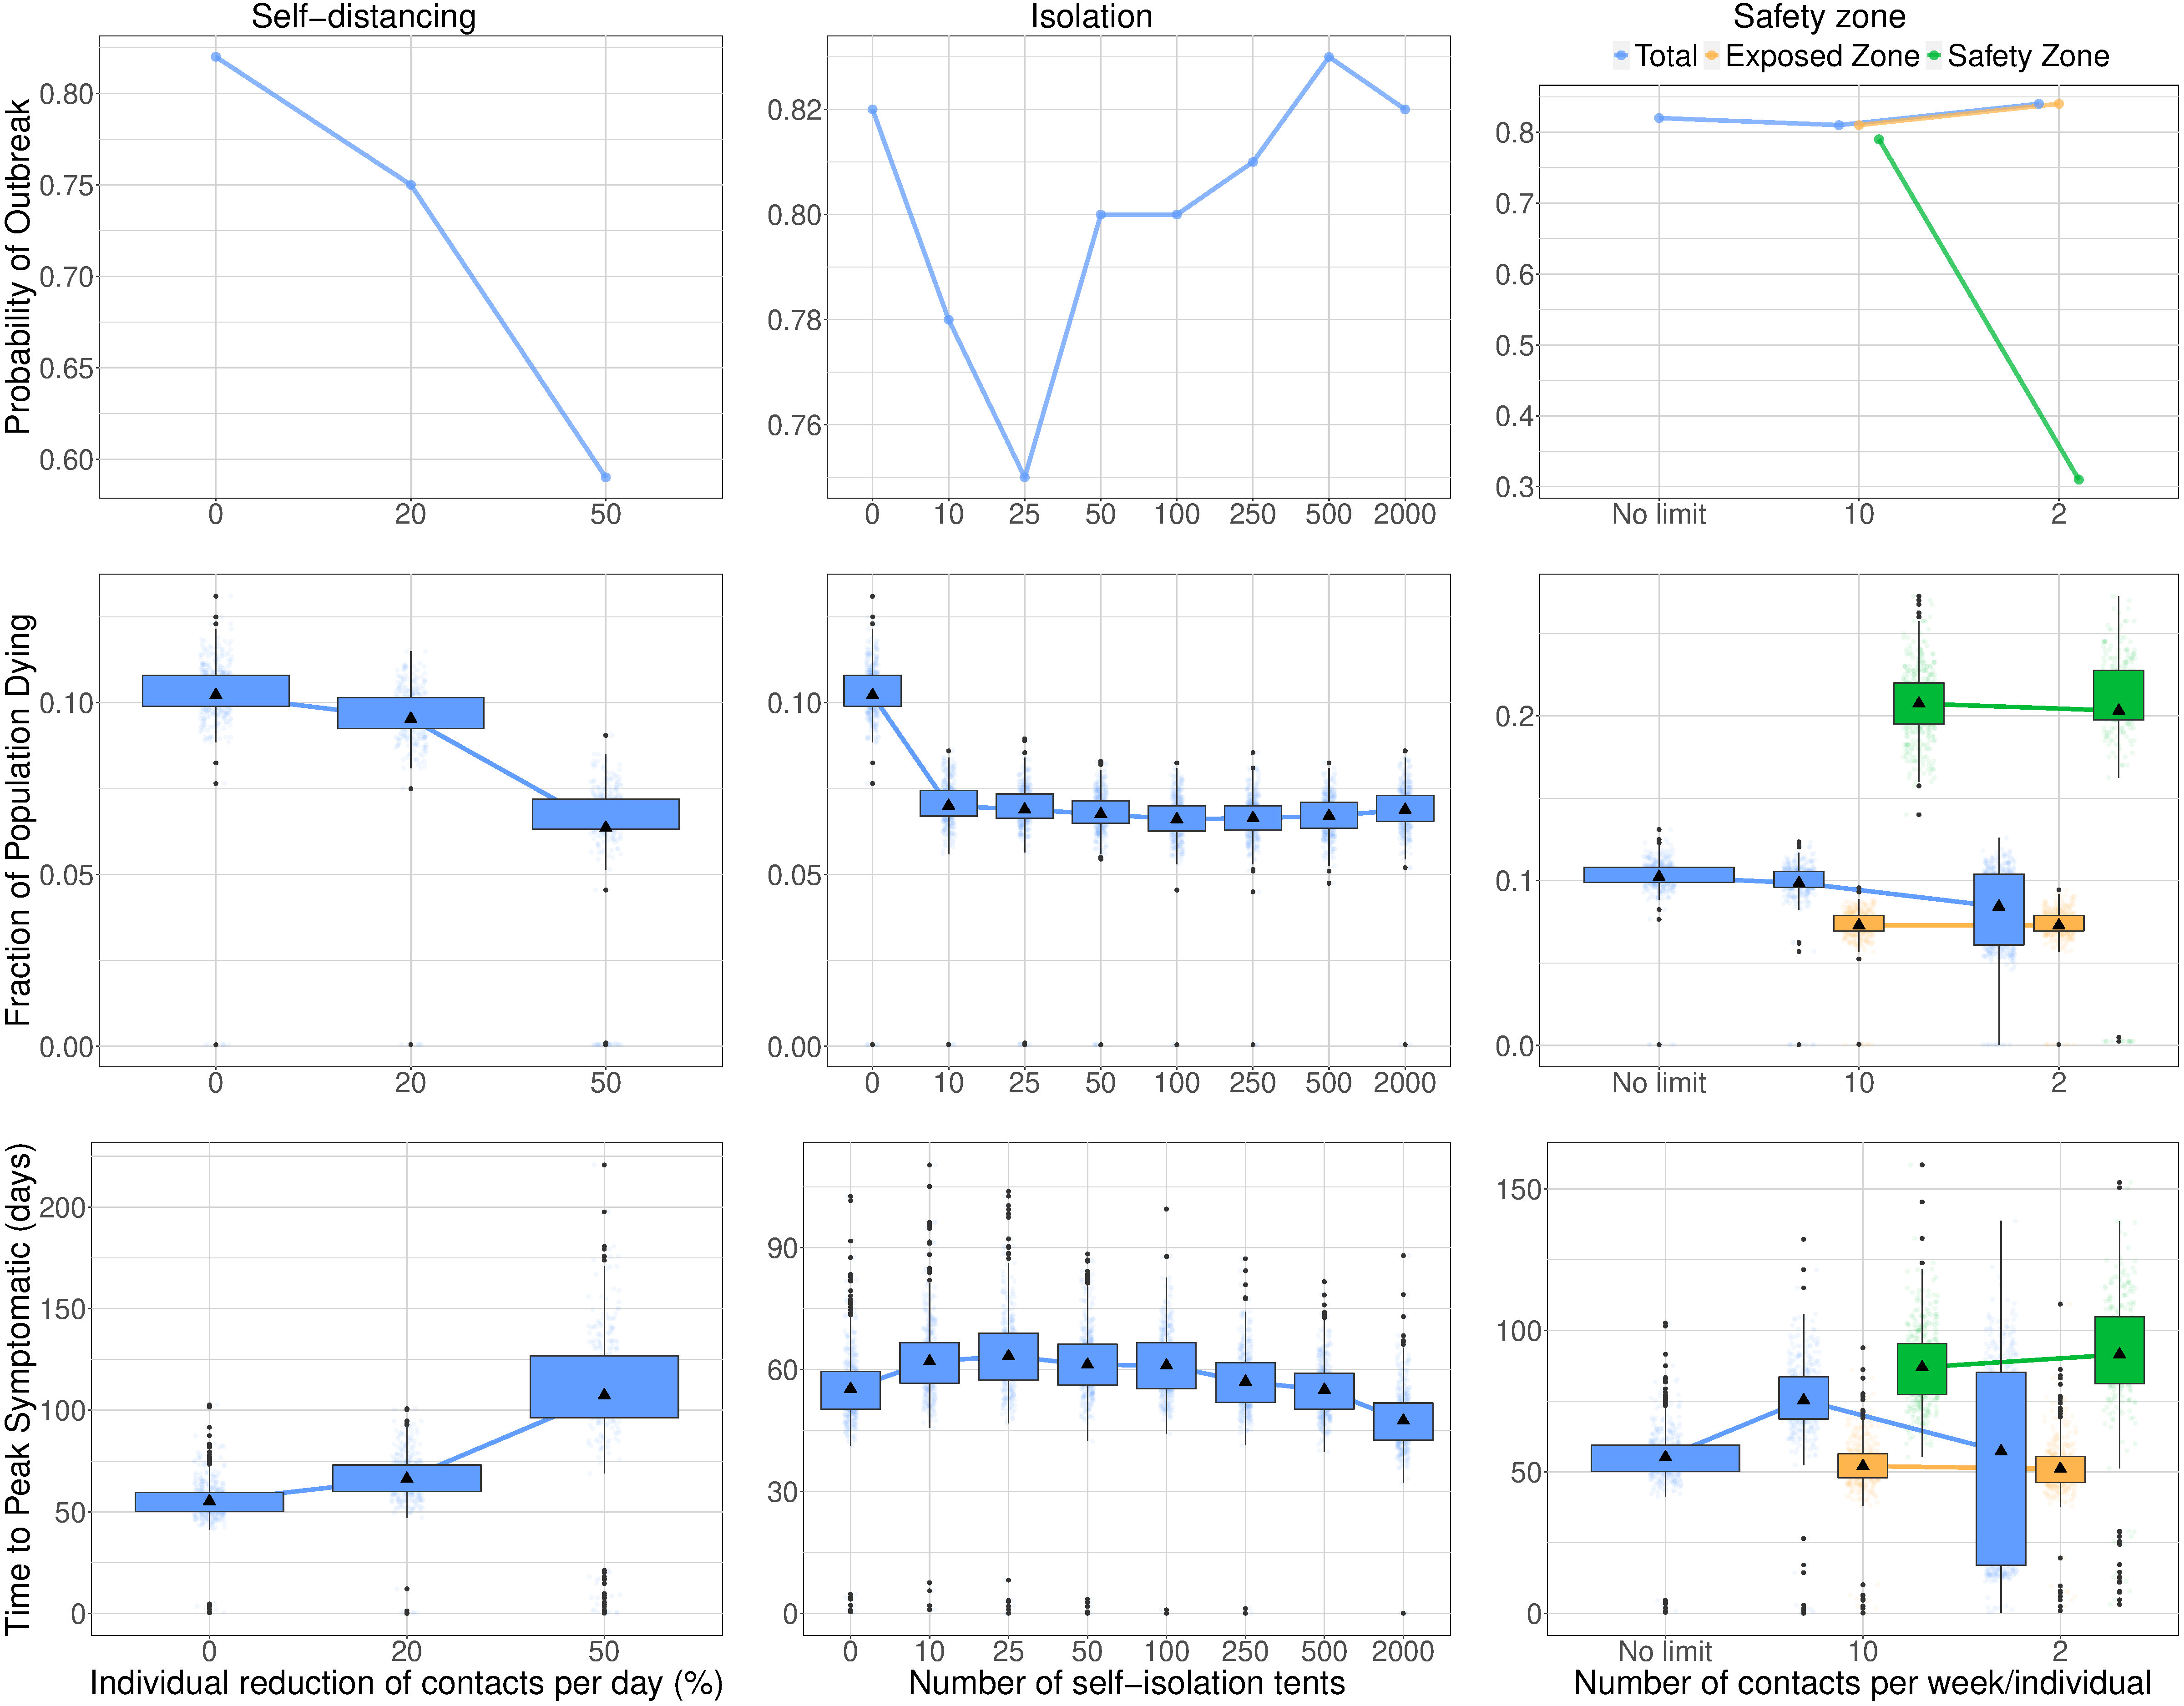
\includegraphics[width=1\textwidth]{figures/Fig2}

\caption{\label{fig:Panel2} \textbf{Effect of interventions on outbreak probability,
fatalities and time until symptomatic cases peak.} A: Self-distancing,
probability of an outbreak. B: Self-distancing, fraction of the population
dying. C: Self-distancing, time until peak symptomatic cases. D: Self-isolation,
probability of an outbreak. E: Self-isolation, fraction of the population
dying. F: Self-isolation, time until peak symptomatic cases. G: Safety
zone, probability of an outbreak. H: Safety zone, fraction of the
population dying. I: Safety zone, time until peak symptomatic cases.
Triangles indicate the means and boxes interquartile ranges. Note
that in figures of the safety zone intervention (panels G-I), the
mean of an outcome for the whole population is not the weighted mean
of the exposed and safety zones, since outcomes are computed considering
simulations in which at least one death was observed in the population
class inhabiting the zone, i.e. the number of simulations considered
to compute each mean is different. In the safety zone figures (panels
G-I) health-checks are in place, in Supplementary Fig. \ref{fig:Suppl_Tcheck}
we show the effect of removing health-checks.}
\end{figure*}


\subsection*{Self-isolation}

With only 10 tents for a camp of 2000 people (i.e. 1 tent for every
200 people), self-isolation yields a marked decrease in the probability
of outbreak ($\sim$26\%) (see Fig. \ref{fig:Panel2}D) but there
is no significant reduction in the mortality (see Fig. \ref{fig:Panel2}E),
suggesting that with a low number of tents the intervention is only
effective in isolating index cases preventing the epidemic to start.
It is needed to further increase the number of tents past this level
up to at least 1 tent for every 8 people to observe a reduction of
$\sim$18\% in the mortality and an increase of $\sim$16\% in the
time to peak of symptomatic individuals. Increasing the number of
tents does not further reduce the probability of outbreak. There is
also an increase in the number of susceptible individuals at the end
of the simulation with increasing number of tents. We finally observed
an artificial increase in the IFR explained by an increasingly large
number of simulations in which very few individuals are infected since,
if at least one of them dies, we retrieve a high IFR value (see Suppl.
Fig. \ref{fig:Suppl_isolation}).

\subsection*{Safety zone}

In this section, we consider the scenario in which all older adults,
younger adults with comorbidities and their family members up to 20\%
of the camp population live in the green zone, unless otherwise specified.
Creating a green zone improves the effect of the previous interventions
overall, but with sometimes opposite outcomes in the exposed and protected
populations. For example, the probability of an outbreak decreases
for the protected population, by around 11\%, if only two contacts
are allowed per week in the buffer zone (see Fig. \ref{fig:Panel2}G).
Notably, most of this reduction is only achieved when health-checks
excluding symptomatic individuals from the buffer zone are in place
(see Supplementary Fig. \ref{fig:Suppl_Tcheck} for the effect of
removing health-checks). On the other hand, the probability of an
outbreak may slightly increase for the exposed population, a consequence
of the relative increase in intra-zone contacts. By shifting the burden
of an outbreak towards the less vulnerable population in the orange
zone, another important outcome of this intervention is the notable
increase in time (62\%) until the number of symptomatic cases peaks
for the vulnerable population, and a 40\% increase in time for the
whole population (see Fig. \ref{fig:Panel2}I). Nevertheless, this
intervention only has a modest reduction on overall mortality (see
Fig. \ref{fig:Panel2}H), possibly due to the high infectiousness
of presymptomatic individuals.

Considering different scenarios for allocating people to the green
zone, the lowest probability of an outbreak is achieved when only
older adults or at most older adults and younger adults with comorbidities
move there, with probabilities below 0.4 and 0.65, respectively (see
Supplementary Fig. \ref{fig:Suppl_popClass}). Positive effects of
the safety zone intervention are even more marked in camps with smaller
populations, especially for probability of an outbreak in the green
zone (which decreases by 55\%) and overall mortality (which decreases
by 20\%) when the population is reduced from 2000 to 500. However,
we also observe the adverse effect of a decrease in time until symptomatic
cases peak (see Supplementary Fig. \ref{fig:Suppl_popSize}). The
incorporation of a lockdown has the greatest effect on reducing the
probability of an outbreak in the green zone, to under 0.25 when contacts
in the buffer zone are reduced by 90\%. While lockdowns show no positive
effect on green zone fatalities in the few instances where an outbreak
does reach there, they decrease overall IFR and fatalities by further
concentrating outbreaks in the less vulnerable population (see Supplementary
Fig. \ref{fig:Suppl_lockdown}).

\subsection*{Evacuation}

We observe no significant effects when severe cases requiring hospitalization
are evacuated (see Supplementary Fig. \ref{fig:Suppl_evacuation}).
Since we considered that these individuals will not receive health
care (they are evacuated to isolation centers), their fate remains
the same than if staying in the camp and, hence, we expect evacuation
to have an effect only in reducing the infectivity. Although these
individuals spend a longer period being infectious with respect to
an individual having mild symptoms ($\sim$10 days longer), the number
of individuals under these conditions is only a small fraction of
the total infectious population at any given time, which explains
why we do not observe significant effects for this intervention.

\subsection*{Combined interventions}

The effects of the interventions observed when we examine them individually
build upon each other when multiple interventions are implemented
in tandem (see Fig. \ref{fig:Panel3} and Supplementary Fig. \ref{fig:Suppl_combined}).
The protective effects of the safety zone intervention especially
are most fully realized not when implemented on its own, but when
paired with other interventions. They become so effective that outbreaks
in the green zone become exceptionally rare, but so well controlled
when they do happen, that the majority of outbreaks are small enough
for us to observe an anomalous increase in IFR in some of the most
effective interventions, driven by the discretization of the values
it can take (e.g. if there is only one case and this person dies,
see Supplementary Table. \ref{fig:Suppl_combined}). When all interventions
are implemented together: strict self-distancing (50\% reduction in
contacts), self-isolation of symptomatic cases (1 tent for every 40
people), a safety zone with 2 contacts per week in the buffer zone,
health checks, a strict lockdown (90\%), and evacuation of severe
cases, mortality is reduced by $\sim$94\% and the probability of
outbreak in the green zone is very small ( $\sim$0.005). In other
combinations with higher probability of outbreak (e.g. considering
in the previous combination a 20\% reduction in contacts instead of
50\%) thetime to peak of symptomatic cases in the green zone is delayed
by 48 days
\begin{figure*}
\begin{centering}
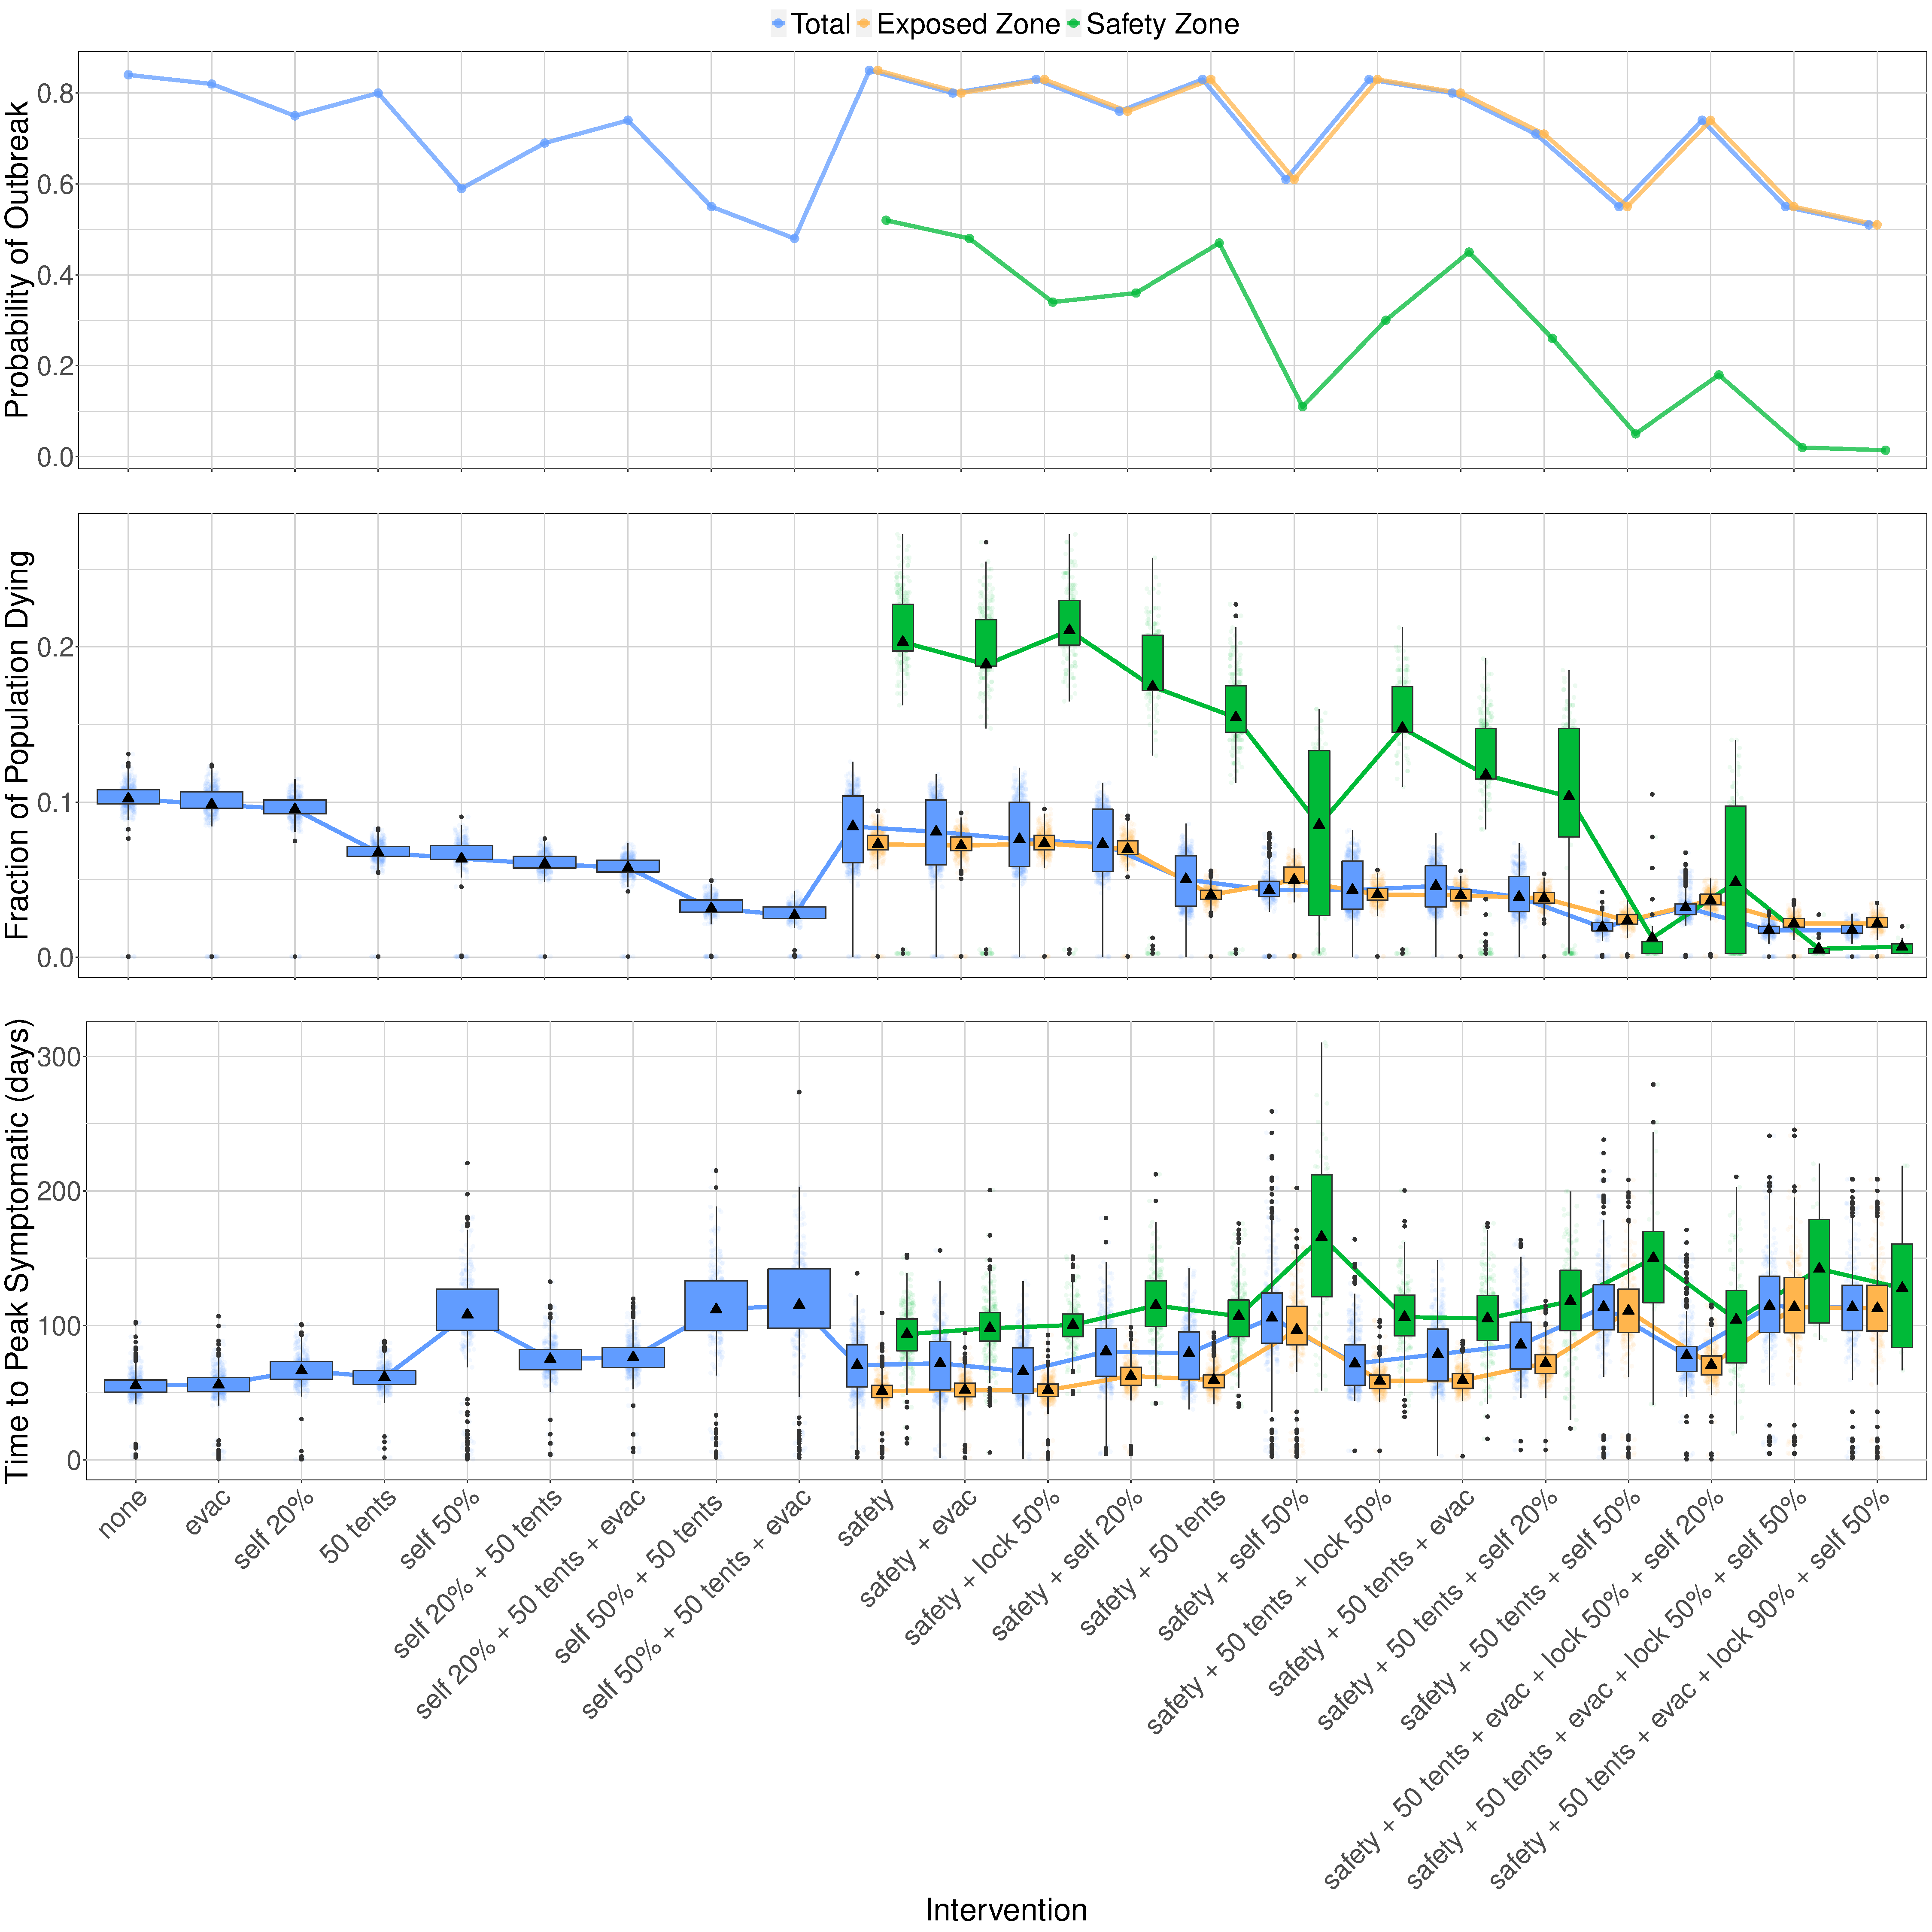
\includegraphics[width=1\textwidth]{figures/Fig3}\\
\par\end{centering}
\caption{\label{fig:Panel3} \textbf{Combinations of interventions.} Probability
of an outbreak (top), fraction of the population dying (middle) and
time until peak symptomatic cases (bottom) for different combination
of interventions. Evac = evacuation of severely symptomatic, self
= self-distancing, tents = number of available self-isolation tents,
safety = safety zone, lock = lockdown of the buffer zone. For combinations
of interventions including a safety zone, we distinguish between the
population living in the green zone, in the orange zone and the whole
population.}
\end{figure*}


\section*{Discussion}

In this study, we propose a number of interventions of immediate applicability
to informal settlements. We focused on IDP settlements in NW Syria,
taking into account the interventions' feasibility, cultural acceptance
and their need for low-cost. When confronted with different possible
scenarios, we generally considered the worst-cases, highlighting the
interventions that are most effective in the direst conditions, but
possibly resulting in an overestimate of mortality. This potential
overestimation does not change the qualitative picture of the results,
which is built upon comparison of relative values between the presence
and absence of interventions.

Our results align with previous simulation studies of potential COVID-19
interventions in similarly densely populated, low-resource settings
where informal settlements are present, such as urban areas of sub-Saharan
Africa. In these settings, social-distancing is demonstrated to be
an effective intervention, and even small changes are estimated to
have large effects on outbreaks \cite{nyabadza2020}, in some cases
determining whether or not already inadequate healthcare systems become
overwhelmed \cite{siraj_early_2020}. Zandvoort et al. show that similar
measures to the ones we consider: self-isolation, physical distancing
and ``shielding'' the vulnerable, may reduce mortality by 60\%-75\%
in African cities \cite{vanzandvoort2020}.

Self-distancing proves to be an effective measure in our models as
well; reducing contacts by 50\% has the greatest effect across most
outcomes of interest in any of the interventions we examined. However,
the difficulty of achieving a reduction of this magnitude cannot be
overlooked, especially considering the large proportion of the population
composed of children, a group with an already high contact rate that
may prove difficult to control \cite{noauthor_syrian_nodate}. To
illustrate the micro-dynamics of this intervention, in Supplementary
Fig. \ref{fig:critical_threshold} we plot the maximum proportion
of the population exposed at any given point in time in each simulation,
against the time it takes for symptomatic cases to peak. We observe
that until reaching approximately 60\%, successive reductions in contacts
reduce the maximum proportion of the population exposed while increasing
the time until symptomatic cases peak. Additional reductions in contacts
beyond 60\% however abruptly decrease both the time until cases peak
and overall mortality, suggesting that outbreaks die out before the
virus spreads widely throughout the camp's population. This suggests
the existence of a critical threshold for the number of individuals
exposed over which large outbreaks become established in the population,
significantly increasing mortality.

We also propose self-isolation using individual tents which can be
located in a dedicated zone or next to the tents of relatives, where
contact with non-isolated individuals is mediated by a buffer zone.
This intervention is effective with even a small number of isolation
tents, as low as 5-10 tents per 1000 camp residents in preventing
an outbreak in the camp, but it requires at least 125 tents per 1000
camp residents to substantially reduce mortality After conversations
with camp managers, we found that this intervention is more likely
to be accepted in NW Syria than evacuation to community-based isolation
centers. Community-based isolation not only poses cultural challenges;
the capacity required to implement it has hardly been met \cite{UNOCHA_CCTC_numbers},
and it is still one of the main challenges in the region \cite{UNOCHA_collapse}.
We note that in our simulated intervention individuals become isolated
as soon as they have symptoms. Recognizing symptoms, however, may
require some time and we should expect a less effective intervention
unless systematic checks for symptomatic individuals are put in place.

Setting up a safety zone has two positive effects that most stand
out: a reduction in the probability of an outbreak in the vulnerable
population, and an increase in the time until the number of symptomatic
cases peaks. Much of the success or failure of the safety zone intervention
hinges on the functioning of the buffer zone. The number of inter-zone
contacts per week, the implementation of health checks, and potential
lockdowns all have notable effects. Also important is the portion
of the population that is protected; protecting only the vulnerable
may have the most beneficial effects, but it is precisely these vulnerable
individuals, older adults and people with comorbidities, who may most
need family members to care for them. While safety zone scenarios
that allow greater numbers of family members to accompany their vulnerable
relatives to the green zone may confer greater epidemiological risk,
they may also engender greater well-being and social cohesion.

Despite these benefits, we do not observe a clear decrease in IFR
with this intervention, although it is possible that our model may
overestimate mortality from an outbreak in the green zone in the few
instances when there is one. Since it is unlikely that the camps have
the economic means to increase the number of tents when implementing
this intervention, we assumed that individuals do not reduce their
contacts when moved to the green zone since household sizes will not
decrease, which implies an increase in the number of contacts between
vulnerable individuals. Despite this increase in contacts, we do not
observe an increase in mortality in the vulnerable population when
the safety zone is implemented. These results address concerns raised
around this type of intervention from previous experiences with large
numbers of fatalities registered in nursing-homes in developed countries
\cite{dahab_covidIDPcontrol_2020}. While nursing-homes in developed
countries may be seen as analogous to the safety zone intervention,
the alternative to nursing homes in developed countries for the elderly
population typically involves remaining at home with few contacts
with younger individuals (in a scenario of lockdown), while in the
camps the alternative is living in tents shared with younger individuals
with high contacts rates (especially children). This may explain why
we observe a positive effect from this intervention despite a relative
increase in contacts among the more vulnerable subpopulation.

An instrumental consideration for our models is the fraction of the
population recovered from COVID-19 after a steady state is reached.
Although the duration for which SARS-CoV-2 infection confers immunity
is uncertain, the proportion of the population recovered after an
outbreak should play a role in its protection against future ones.
For all intervention except self-distancing \textgreater 30\%, we
observed that the fraction of the population recovered meets or exceeds
50\%.

Another important consideration for interpreting our results are the
modelling assumptions we made. From the point of view of our parameterization,
perhaps the most relevant relates to the relative transmissivity of
the different infectious stages, whose specific values still have
large margins of variability \cite{widders_viralLoadVsInfect_2020,casey_presymptEstim_2020,he_temporal_2020}.
This is particularly relevant for our purposes, because the higher
the relative infectivity of the presymptomatic and asymptomatic stages,
the less effective our non-medical interventions which rely on identification
of symptomatic individuals will be. For instance, Bullock et al. \cite{bullock_IBM4IDPs_covid21}
assumed a higher infectiousness of the presymptomatic stage and hence
self-isolation of symptomatic individuals had little effect. Self-isolation
also becomes ineffective under the assumptions made by Hernandez-Suarez
et al. \cite{hernandez_Refugee_covid20} when they considered isolating
only severe symptomatic cases (whose fraction is small), hence mildly
symptomatic individuals were effectively considered asymptomatic.
On the other hand, Gilman et al. \cite{gilman_IBMrefugee_covid20}
showed that self-isolation was effective when considering individuals
at different stages to be equally infectious. We assumed that presymptomatic
individuals have the highest relative infectivity, consistent with
the most recent estimations \cite{casey_presymptEstim_2020}, and
the interventions we proposed are still effective. Considering a different
scenario in which all compartments are assumed to be equally infectious,
our interventions become even more effective (see previous version
of our manuscript \cite{pascual-garcia_medRxiv_2020}v1).

It is also important to acknowledge the benefits and limitations of
different possible computational implementations. For instance, there
are interventions that do not have a natural implementation within
our framework, such as those requiring interventions targeting very
specific interactions between individuals (as opposed to large groups
of individuals), or reproducing empirically-observed residence times.
An example might be the isolation of an individual and his/her family,
as proposed by Gilman \emph{et al.} \cite{gilman_IBMrefugee_covid20}
which, since we do not explicitly model interactions at the family-level,
would require the creation of as many classes as families. When this
level of detail is required, individual based models (IBMs) may be
more appropriate \cite{gilman_IBMrefugee_covid20,bullock_IBM4IDPs_covid21}.
However, IBMs require a rich amount of data for their parameterization
which, although increasingly available, is scarce for informal IDPs
camps. Our framework is powerful enough to simulate a large number
of scenarios with little computational cost, which would be an optimal
strategy as a first approximation in the design of interventions to
narrow down the most relevant scenarios (as a reference, in \textless 24h
we model with just 12 cores 75 scenarios requiring quarter million
simulations). The scenarios selected could then be further investigated
with more detailed interventions using IBMs, if data is available.

A key limitation of our approach is that it simulates an outbreak
started by one infectious individual in a single camp with a closed
population. We acknowledge that this approach does not fully capture
the complexities of the NWS region, where IDPs live interspersed throughout
the region in several hundred camps. The dynamics of an outbreak in
the region are undoubtedly influenced by inter-community contacts,
and the dynamics of an outbreak in a single camp by these region-wide
dynamics, as it has been demonstrated in other countries \cite{gatto_spread_2020,arenas2020}.
We expect our results to be robust to changes in population, as long
as these changes are relatively small compared to the total population
size in the camp, implying sporadic inputs of infected individuals.
This is the expected behaviour in IDPs, which are often small and
located in rural areas, and in which important population movements,
as those observed in large camps, are infrequent. This fact, together
with the relatively young population in IDPs, may help in limiting
the impact of the disease, as observed in African rural areas \cite{diop_COVIDruralAfrica_2020}.

Other unaccounted for social and cultural dynamics will undeniably
complicate the feasibility of our proposed interventions. Only one
example we have not addressed here is the unlikeliness of children
under 13 self-isolating. Although the number of challenges to implementing
our proposed interventions are potentially endless, the community-based
nature of our approach may help circumvent these challenges much faster
than healthcare-based interventions, which often depend on complex
political decisions and may take years to build the requisite capacity
for an effective response. If the dynamics of the virus are well understood
by local communities and at least some of the interventions we propose
are implemented, the impacts of COVID-19 can be mitigated even in
an environment as challenging as NW Syria.

\section*{Conclusion}

Given a rapidly changing environment and slow responses of local and
international authorities in conflict regions where control of policy
is disputed, the latter often leaving these communities aside in their
priorities \cite{Mukumbange_refugeesVaccine_2020}, empowering local
communities themselves is perhaps the best, if not the only way, to
help them avoid the worst consequences of the pandemic. Such an approach
may achieve greater compliance with non-pharmaceutical interventions,
especially where there is a mistrust of external authority. This not
only applies to IDP camps in NW Syria, but more generally to refugee
camps in conflict-torn regions, and potentially other informal settlements
and vulnerable communities around the world: the low-cost, effective
interventions we present are feasible, needed and urgent.

\section*{Acknowledgements}

This collaboration was organized by crowdfightCOVID19 (www.crowdfightcovid19.org)
upon request from CS. We thank Judith Boumann for valuable contributions.
We thank Peter Ashcroft, Juan Poyatos, Noreen Goldman, Burcu Tepekule
and members of Sebastian Bonhoeffer's and Bryan Grenfell's groups
for useful discussions. We thank two anonymous reviewers who provided
thoughtful and insightful comments that greatly improved our article.

\section*{Declarations}

\subsubsection*{Funding}

ECF's research is supported by Wellcome Trust grant 204833/Z/16/Z.
APG research is supported by the Simons Collaboration: Principles
of Microbial Ecosystems (PriME), award number 542381.

\subsubsection*{Conflicts of interest/Competing interests}

Alberto Pascual-García is a Board Member of crowdfightCOVID19, an
initiative from the scientific community to put all available resources
at service of the fight against COVID-19. Chamsy Sarkis (co-author)
is a Board Member of the Pax Syriana Foundation, a non-profit organization
set up for social and philanthropic purposes including promoting and
providing support and assistance to civilian aid projects in the fields
of education, health, emergency assistance, psychological assistance
and humanitarian aid for people affected by wars or humanitarian crises.
These organizations had no role in study design, data collection,
data analysis, data interpretation, or writing of the article.

\subsubsection*{Ethics approval}

This study used only publicly available aggregate data and was thus
not subject to ethical review.

\subsubsection*{Consent to participate}

NA

\subsubsection*{Consent for publication}

All authors agreed on publication.

\subsubsection*{Availability of data and material}

All results are available at the url https://github.com/crowdfightcovid19/req-550-Syria

\subsubsection*{Code availability}

All the code is freely available at the url https://github.com/crowdfightcovid19/req-550-Syria

\subsubsection*{Authors' contributions}

All authors contributed to the conceptualization. Design of the methodology:
APG, ECF, JV, JK, CS. Formal analysis: APG, ECF, JK. Code development
APG, ECF, JK. Conducted research: APG, ECF, JV, JK. Validate results:
APG, ECF, JK, JV, CS. Contributed resources: APG, CS, ECF, JK, JV.
Data curation: APG, JK, ECF. Visualization: APG, ECF, JK, JV. Writing
(original draft) APG, ECF, JK. All authors contributed to the final
version of the manuscript, and APG supervised the research.

\bibliographystyle{unsrt}
\bibliography{req550-syria}

\end{document}
